\documentclass[10pt,letterpaper]{article}
\usepackage[latin1]{inputenc}
\usepackage{amsmath}
\usepackage{amsfonts}
\usepackage{amssymb}
\usepackage{graphicx}
\usepackage[margin=1in]{geometry}
\usepackage{listings}
\usepackage{float}
\usepackage{fancyhdr}
\pagestyle{fancy}
\lhead{\today}
\chead{Project 3}
\rhead{Tan, Zhou}
%\usepackage[margin=1in]{geometry}
\usepackage{color} %red, green, blue, yellow, cyan, magenta, black, white
\definecolor{mygreen}{RGB}{28,172,0} % color values Red, Green, Blue
\definecolor{mylilas}{RGB}{170,55,241}

\newcommand{\ssbracket}[2]{#1^{(#2)}}

\author{Hao Hui Tan(999741711, tanstev1)\\Kyle Zhou (1000959732, zhoukyle)}
\title{CSC411H1S Project 3}
\begin{document}
	\lstset{language=Python,%
		%basicstyle=\color{red},
		breaklines=true,%
		%morekeywords={matlab2tikz},
		keywordstyle=\color{blue},%
		morekeywords=[2]{1}, keywordstyle=[2]{\color{black}},
		identifierstyle=\color{black},%
		stringstyle=\color{mylilas},
		commentstyle=\color{mygreen},%
		showstringspaces=false,%without this there will be a symbol in the places where there is a space
		numbers=left,%
		numberstyle={\tiny \color{black}},% size of the numbers
		numbersep=9pt, % this defines how far the numbers are from the text
		emph=[1]{for,end,break},emphstyle=[1]\color{red}, %some words to emphasise
		%emph=[2]{word1,word2}, emphstyle=[2]{style},
		caption=\lstname,
	}

	\maketitle
	\newpage
	\begin{enumerate}
		\item %1
		The Real headline data set seems to be larger than the Fake headline data set.
		Most of the headlines for both data sets are in English, but there are some French and Spanish headlines, as well as possibly other languages.

		Fake headlines seem to use ``Trump'' to refer to Donald Trump, while real headlines tend to use ``Donald Trump.''
		Fake headlines also tend to use more sensational or inflammatory terms such as declaring something ``an hilarious fail,'' or have grammatical mistakes like the aforementioned example.
		Headlines in general are all lowercase with no punctuation.
		However, it seems that the real headlines tend to be truncated, while the fake headlines seem to all have the full text.
		Some of the headlines are also misspelled (e.g. ``x jinpingi'' instead of ``xi jinping'').

		It is difficult to categorize headlines solely based on keywords, since the same word in different contexts could be either sensational, or factual.
		Some useful keywords could be ``racist'' (5 occurrences in fake, 2 occurrences in real), ``hillary,'' (18 occurrences in real, 97 occurrences in fake), and ``rigged'' (3 occurrences in real, 15 occurrences in fake).

		\item %2
		The Naive Bayes algorithm was computed by computing the conditional probability 
		\[
			P(x_i | c) =  \frac{count(x_i = 1, c)}{count(c)}
		\]
		for all $x_i$ in the training set, and for each class $c$ (i.e. ``real'' or ``fake'').
		The actual formula used involves using $m$ and $\hat{p}$ as priors in order to improve the accuracy of our model, since many words only occur once, or a few times.
		Thus, the formula we trained with was
		\[
			P(x_i | c) =  \frac{count(x_i = 1, c) + m\hat{p}}{count(c) + m}
		\]
		
		To predict whether a headline was real or fake, we computed the conditional probability
		\[P(x_1, ..., x_n | c) P(c)\]
		by computing 
		\[\prod_{i = 1}^{n}p(x_i|y=c)\]
		However, since for the less frequent words, $p(x_i|y=c)$ is very small, and multiplying them together may result in underflow, we computed the exponential of the sum of the log probabilities instead.
		Thus, our formula becomes 
		\[
			P(x_1, ..., x_n | c) P(c) = \exp\left(\sum_{i = 1}^{n}\log(P(x_i|y=c))\right)P(c)
		\]
		We then return the class with the highest probability as our prediction.
		
		In order to tune the $m$ and $\hat{p}$ parameters, we trained the model with varying values, with $m \in [1, 20]$ and $p\in [0.1, 1.0]$, with a step of 1 and 0.1, respectively, and found the values that performed best on the validation set.
		
		The performance of the classifier on the training set is 96\%, and the performance on the test set is 85\%
		
		The best params are as follows: \\
		\[m = 2, \hat{p} = 0.2\]
		\\
		The code is included below:
		\begin{lstlisting}
def train_model(real_headlines, fake_headlines, m, p):
    word_list = get_wordlist(real_headlines, fake_headlines)
    real_counts = count_word_occurrance(real_headlines)
    fake_counts = count_word_occurrance(fake_headlines)
    probabilities_real = {}
    probabilities_fake = {}
    for word in word_list:
        # if word in ENGLISH_STOP_WORDS: continue
        if word in real_counts:
            probabilities_real[word] = (real_counts[word] + m * p) / float(len(real_headlines) + m)
        else:
            probabilities_real[word] = (0 + m * p) / float(len(real_headlines) + m)
        if word in fake_counts:
            probabilities_fake[word] = (fake_counts[word] + m * p) / float(len(fake_headlines) + m)
        else:
            probabilities_fake[word] = (0 + m * p) / float(len(fake_headlines) + m)

    return probabilities_real, probabilities_fake, m, p, len(real_headlines), len(fake_headlines), word_list

def predict_model(model, headline):
    probabilities_real, probabilities_fake, m, p, real_count, fake_count, word_list = model
    logprob_real = 0.0
    logprob_fake = 0.0
    real_class_prob = float(real_count) / (real_count + fake_count)
    fake_class_prob = float(fake_count) / (real_count + fake_count)
    headline_split = headline.split(' ')
    for word in word_list:
        # if word in ENGLISH_STOP_WORDS: continue
        if word in headline_split:
            logprob_real += math.log(probabilities_real[word])
            logprob_fake += math.log(probabilities_fake[word])
        else:
            logprob_real += math.log(1 - probabilities_real[word])
            logprob_fake += math.log(1 - probabilities_fake[word])
    real_prob = math.exp(logprob_real) * real_class_prob
    fake_prob = math.exp(logprob_fake) * fake_class_prob
    # print real_prob, fake_prob
    return real_prob > fake_prob

def tune_model(real_training, fake_training, real_validation, fake_validation):
    performance_report = {}
    m = 1
    while m <= 20:
        p = 0.1
        while p <= 1:
            model = train_model(real_training, fake_training, m, p)
            performance = get_performance(model, real_validation, fake_validation)
            print m, p, performance
            performance_report[(m, p)] = performance
            p += 0.1
        m += 1

    print "The m and p value is", max(performance_report, key=performance_report.get)

    return performance_report

def get_performance(model, real, fake):
    correct = 0

    for hl in real:
        if predict_model(model, hl):
            correct += 1

    for hl in fake:
        if not predict_model(model, hl):
            correct += 1

    return float(correct) / (len(real) + len(fake))
		\end{lstlisting}
		\item %3
		\begin{enumerate}
			\item %3a
			The 10 words whose presence most strongly predicts that the news is real
			\begin{enumerate}
				\item japan
				\item daniel
				\item refugee
				\item denies
				\item zoe
				\item charlottesville
				\item korea
				\item business
				\item nfl
				\item south
			\end{enumerate}
			
			The 10 words whose absence most strongly predicts that the news is real
			\begin{enumerate}
				\item trump
				\item the
				\item to
				\item hillary
				\item a
				\item is
				\item and
				\item for
				\item clinton
				\item in
			\end{enumerate}
			
			The 10 words whose presence most strongly predicts that the news is fake
			\begin{enumerate}
				\item hats
				\item debunks
				\item sleep
				\item hating
				\item battleground
				\item haters
				\item pointing
				\item dazu
				\item pantano
				\item amtsantritt
			\end{enumerate}
			
			The 10 words whose absence most strongly predicts that the news is fake
			\begin{enumerate}
				\item donald
				\item trumps
				\item us
				\item says
				\item ban
				\item korea
				\item north
				\item turnbull
				\item travel
				\item australia
			\end{enumerate}
		
			These lists were obtained by finding the words with the max values for the conditional probabilities
			\[
				P(\text{class} | \text{word}) = \frac{P(\text{word} | \text{class})P(\text{class})}{P(\text{word})}
			\]
			where
			\[
				P(\text{word}) = \frac{\text{count}(\text{word}) + m\hat{p}}{\text{\text{count}}(\text{headlines}) + m}
			\]
			and
			\[
			P(\text{class} | \neg\text{word}) = \frac{P(\neg\text{word} | \text{class})P(\text{class})}{P(\neg\text{word})}
			\]
			\[
			= \frac{(1 - P(\text{word} | \text{class}))P(\text{class})}{1 - P(\text{word})}
			\]
			The words that have the biggest sway on whether a headline is real or fake tend to be words that only appear in one set and not the other.
			However, the presence of a word in one class's top 10 doesn't imply that it will be as strong when absent from the other class.
			
			
			%(model.probs_real[k] * prob_real) / (model.real_word_counts[k] + model.m / float(model.real_word_counts[k] + model.fake_word_counts[k]))
			%If the conditional probability is high, then if the word is present in the headline, it will not decrease the term $P(x_1, ..., x_n | c)$ as much (since the probability is closer to 1), which means that the final conditional probability will be higher.
			%If the conditional probability is low, then if the word is \textit{absent} from the headline, it will also result in a lower penalty than if the probability were higher.
			%That's because $1 - P(x_i|c)$ is used instead.
			For the code, please see \verb|get_top_bottom_word_occurrences| in fake.py.
			
			%However, due to the addition of the $m$ and $\hat{p}$ values to the equation for $p(x_i|c)$, the bounds on the probability is not 1.0 and 0.0.
			%In the case of our optimal values ($m = 2, \hat{p} = 0.2$), the min and max values are  0.00392 and 0.984, respectively.
			%Since \(1 - 0.00392 > 0.984\), having a missing word absent is stronger than having a common word present.
			
			\item %3b
			The following lists have had the stopwords from scikit\_learn excluded
			
			The 10 words whose presence most strongly predicts that the news is real
			\begin{enumerate}
				\item japan
				\item daniel
				\item refugee
				\item denies
				\item zoe
				\item charlottesville
				\item korea
				\item business
				\item nfl
				\item south
			\end{enumerate}
			
			The 10 words whose absence most strongly predicts that the news is real
			\begin{enumerate}
				\item trump
				\item hillary
				\item clinton
				\item just
				\item america
				\item supporters
				\item vote
				\item black
				\item win
				\item watch
			\end{enumerate}
			
			The 10 words whose presence most strongly predicts that the news is fake
			\begin{enumerate}
				\item hats
				\item debunks
				\item sleep
				\item hating
				\item battleground
				\item haters
				\item pointing
				\item dazu
				\item pantano
				\item amtsantritt
			\end{enumerate}
			
			The 10 words whose absence most strongly predicts that the news is fake
			\begin{enumerate}
				\item donald
				\item trumps
				\item says
				\item ban
				\item korea
				\item north
				\item turnbull
				\item travel
				\item australia
				\item climate
			\end{enumerate}
			\item %3c
			It might make sense to remove stopwords when looking at the ratio of word frequency between the real and fake headlines, because these words are common, and would likely appear in most if not all headlines.
			These words are also uninteresting on their own, and so they crowd up the word frequency rankings, possibly pushing more interesting words down the list.
			Another reason for removing stopwords would be when the input set includes headlines of different languages.
			This is because stopwords in one language are usually uncommon in other languages, and once again skew the results.
			
			It would make sense to keep stopwords because their presence could still help distinguish between classes, because one class might use certain stopwords in a different way, or use them more (or less) frequently than the other class.
			Furthermore, in testing, we have found that training while excluding stopwords does not necessarily increase the performance of our model.
			
		\end{enumerate}
	\item %4
	The learning curves of Logistic Regression can be seen in Figure \ref{fig:part4learningcurve}.
	\begin{figure}[H]
		\centering
		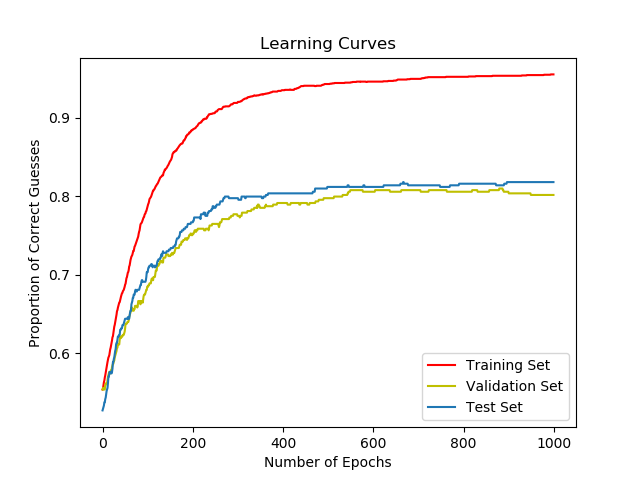
\includegraphics[width=\linewidth]{Part4LearningCurve}
		\caption{Performance of Logistic Regression vs. Number of Epochs}
		\label{fig:part4learningcurve}
	\end{figure}
	
	% talk about how you chose the regularization parameter
	\item %5
	\item %6
	\begin{enumerate}
		\item %6a
		\item %6b
		\item %6c
	\end{enumerate}
	\item %7
	\begin{enumerate}
		\item %7a
		\item %7b
		\item %7c
	\end{enumerate}
	\item %8
	\begin{enumerate}
		\item %8a
		\item %8b
	\end{enumerate}
	\end{enumerate}
\end{document}
